\documentclass[a4paper,12pt]{article} 

%%% Работа с русским языком
\usepackage{cmap}					% поиск в PDF
\usepackage{mathtext} 				% русские буквы в фомулах
\usepackage[T2A]{fontenc}			% кодировка
\usepackage[utf8]{inputenc}			% кодировка исходного текста
\usepackage[english,russian]{babel}	% локализация и переносы

%%% Дополнительная работа с математикой
\usepackage{amsmath,amsfonts,amssymb,amsthm,mathtools, gensymb} % AMS
\usepackage{icomma} % "Умная" запятая: $0,2$ --- число, $0, 2$ --- перечисление

%%Таблица
\usepackage[table,xcdraw]{xcolor}
\usepackage{caption}
\usepackage{subcaption}
\usepackage{floatrow}
\floatsetup[table]{capposition=top}
\floatsetup[wrapfigure]{capposition=bottom}
%multi-column
%\usepackage{multi-column}
%multi-row
\usepackage{multirow}


%% Номера формул
\mathtoolsset{showonlyrefs=true} % Показывать номера только у тех формул, на которые есть \eqref{} в тексте.

%% Шрифты
\usepackage{euscript}	 % Шрифт Евклид
\usepackage{mathrsfs} % Красивый матшрифт

%% Свои команды
\DeclareMathOperator{\sgn}{\mathop{sgn}}

%% Перенос знаков в формулах (по Львовскому)
\newcommand*{\hm}[1]{#1\nobreak\discretionary{}
{\hbox{$\mathsurround=0pt #1$}}{}}

%% Стиль страницы
\usepackage{fancyhdr}

%% Для рисунков
\usepackage{graphicx}
\usepackage[export]{adjustbox}
\usepackage{float}
\usepackage{ragged2e}
\usepackage{wrapfig}

%Отступы и поля 
\textwidth=20cm
\oddsidemargin=-2cm
\topmargin=-2cm
\textheight=25cm

\pagestyle{fancy}
\begin{document}
\begin{titlepage}
\begin{center}
%\vspace*{1cm}
\large{\small ФЕДЕРАЛЬНОЕ ГОСУДАРСТВЕННОЕ АВТОНОМНОЕ ОБРАЗОВАТЕЛЬНОЕ\\ УЧРЕЖДЕНИЕ ВЫСШЕГО ОБРАЗОВАНИЯ \\ МОСКОВСКИЙ ФИЗИКО-ТЕХНИЧЕСКИЙ ИНСТИТУТ\\ (НАЦИОНАЛЬНЫЙ ИССЛЕДОВАТЕЛЬСКИЙ УНИВЕРСИТЕТ)\\ ФАКУЛЬТЕТ АЭРОКОСМИЧЕСКИХ ТЕХНОЛОГИЙ}
\vfill
\line(1,0){430}\\[1mm]
%\huge{Лабораторная 2}\\
\huge\textbf{Определение критической силы при потери устойчивости стержней}\\
\line(1,0){430}\\[1mm]
\vfill
\begin{flushright}
\normalsize{Рогозин Владимир}\\
\normalsize{\textbf{Группа Б03-106}}\\
\end{flushright}
\end{center}
\end{titlepage}
\fancyhead[c] {Определение критической силы при потери устойчивости стержней}

\textbf{Цель работы:} 
1) Ознакомление с основными положениями теории устойчивости стержней по Эйлеру. \\
2) Проведение экспериментов и сопоставление расчётных и экспериментальных данных. 

\textbf{Теоретические сведения:}
Рассмотрим изгиб однородного бруса (балки) произвольного постоянного поперечного сечения на рис. 1. Ввиду бесконечной малости выделенного элемента можно считать, что в результате изгиба прямые $АА', NN', ВВ'$ и все прямые, им параллельные, перейдут в окружности с центрами, лежащими на оси О, перпендикулярной к плоскости рисунка.

\begin{figure}[H]\label{fig:izgib} 
    \centering
    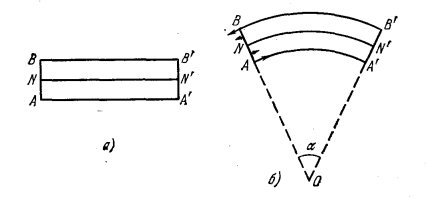
\includegraphics[width = \textwidth]{Izgib.png}
    \caption{а) Балка в покоящемся состоянии, б) изогнутая балка}
\end{figure}
 Эта ось называется осью изгиба. Наружные волокна, лежащие выше
линии $NN'$, при изгибе удлиняются, волокна, лежащие ниже линии $NN
'$, — укорачиваются. Длина линии $NN'$ остается неизменной. Эта линия называется \textit{нейтральной} линией. Проходящее через нее сечение (недеформированного) бруса плоскостью, перпендикулярной к плоскости рисунка называется \textit{нейтральным} сечением. Пусть $R$ — радиус кривизны нейтральной линии. Рассмотрим удлинение волокна бруса, находящегося на расстоянии $\xi$ от нейтральной линни.  Если брус не слишком толст, так что $|\xi| \ll R$, то длина рассматриваемого волокна будет $l = (R + \xi) \alpha$, а удлинение $\Delta l = l - l_0 = \xi \alpha$. Получаем натяжение вдоль рассматриваемого волокна 
\[\tau = E \frac{\xi}{R}\]
отсюда момент сил, действующий на брусок относительно оси, перпендикулярной рисунку и проходящей через середину нейтральной линии
\[M_\tau = \frac{E}{R}\int \xi^2 dS = \frac{EJ}{R}\]
где обозначен осевой момент инерции
\[J = \int \xi^2 dS\]
Вспоминая выражение для радиуса кривизны
\[\frac{1}{R} = \frac{y''}{(1 + (y')^2)^{3 / 2}}\]
при малых изгибах можно пренебречь квадратом производной. Окончательно запишем выражение для момента сил, действующих внутри стержня
\[M_\tau = EJy''\]
\begin{figure}\label{fig: izgibMoment}
    \centering
    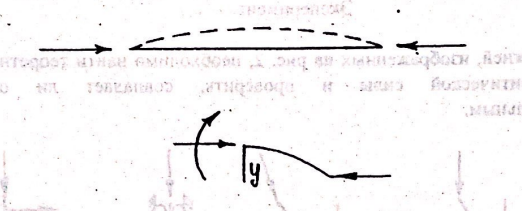
\includegraphics[width = 0.8\textwidth]{IzgibMoment.png}
    \caption{Изгиб стержня под действием внешнего момента}
\end{figure}

Внешний момент силы $P$ равен 
\[M = -Py\]
получаем уравнение 
\[y'' + k^2 y = 0, \quad k^2 = \frac{P}{EJ}\]
Общее решение данного уравнения представляется в виде
\[ y = A\sin kx + B\cos kx\]
где $A, B$ - произвольные постоянные, которые могут быть вычислены из граничных условий
\[x = 0, \text{ } y = 0; \quad x = l, \text{ } y = 0\]
окончательный результат 
\[B = 0, \quad A\sin kl = 0\]
Случай $A = 0$ соответствует состоянию устойчивости. Потеря устойчивости происходит при условии 
\[kl = \pi n\text{, где $n$ -- целое число.}\] 
Выражая силу получим 
\[P = \frac{\pi^2 n^2 E J}{l^2}\]
беря наименьшее значение $n$ получаем выражение для критической силы
\[P_{кр} = \frac{\pi^2 E J}{l_{эфф}^2}\]
Так как изначально формула была получена для шарнирно закреплённого с двух сторон стержня, то при изменении способа закрепления концов должно меняться и значение критической силы, это и отражает переменная в знаменателе $l_{эфф} = \mu l$, где $l$ -- фактическая длина стержня, $\mu$ -- коэффициент, показывающий во сколько раз критическая сила при данном закреплении меньше критической силы при двойном шарнирном крепеже для стержней одинаковой длины. 
\newpage

\begin{figure}[H]\label{fig: sterjni}
    \centering
    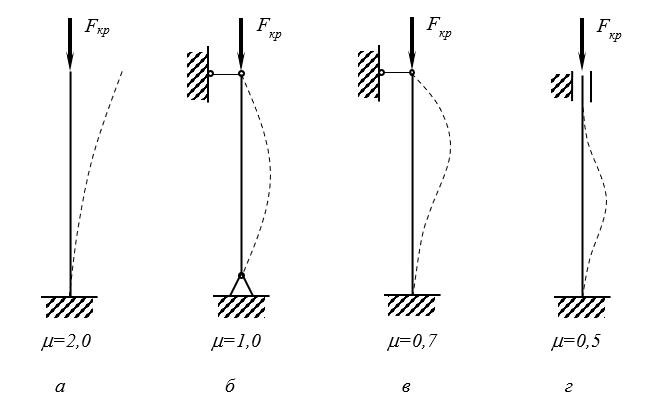
\includegraphics[width = \textwidth]{Sterjni.png}
    \caption{Значения коэффициента $\mu$ для различных способов закрепления стержня}
\end{figure}

\textbf{Обработка данных:} В данной работе рассчитывалась критическая сила для каждого из четырех представленных выше способов крепления стержня. Длины каждой из линеек, а также их коэфиициенты $\mu$ представлены на схеме ниже. Параметры каждой из линеек:
\[b_I = 2,81 \text{ $см$}, \quad b_{II} = 3,59 \text{ $см$}, \quad h_1 = h_2 = h = 0,95 \text{ $мм$} \quad E = 2 \cdot 10^{6} \text{ $кг / см^2$}\]
где $b_I, b_{II}$ -- высоты ближней и дальней линеек соответственно, $h$ -- их толщина, $E$ -- модуль Юнга стали.

Осевой момент инерции рассчитывается по формуле
\[J = \int \xi^2 dS = \frac{b h^3}{12}\]
\begin{table}[H]\label{tab: DataAndJ}
    \centering
    \begin{tabular}{|c|c|c|c|c|}
        \hline
        {\color[HTML]{000000} №}    & {\color[HTML]{000000} $l, см$} & {\color[HTML]{000000} $b, см$} & {\color[HTML]{000000} $\mu$} & {\color[HTML]{000000} $J, см^4$} \\ \hline
        {\color[HTML]{000000} I.1}  & {\color[HTML]{000000} 23,1}  & {\color[HTML]{000000} }      & {\color[HTML]{000000} 2,0} & {\color[HTML]{000000} }        \\ \cline{1-2} \cline{4-4}
        {\color[HTML]{000000} I.2}  & {\color[HTML]{000000} 26,7}  & {\color[HTML]{000000} }      & {\color[HTML]{000000} 0,7} & {\color[HTML]{000000} }        \\ \cline{1-2} \cline{4-4}
        {\color[HTML]{000000} I.3} &
          {\color[HTML]{000000} 31,8} &
          \multirow{-3}{*}{{\color[HTML]{000000} 2,81}} &
          {\color[HTML]{000000} 1,0} &
          \multirow{-3}{*}{{\color[HTML]{000000} $2,007 \cdot 10^{-4}$}} \\ \hline
        {\color[HTML]{000000} II.4} & {\color[HTML]{000000} 46,5}  & {\color[HTML]{000000} }      & {\color[HTML]{000000} 0,5} & {\color[HTML]{000000} }        \\ \cline{1-2} \cline{4-4}
        {\color[HTML]{000000} II.5} &
          {\color[HTML]{000000} 32,8} &
          \multirow{-2}{*}{{\color[HTML]{000000} 3,59}} &
          {\color[HTML]{000000} 0,7} &
          \multirow{-2}{*}{{\color[HTML]{000000} $2,564 \cdot 10^{-4}$}} \\ \hline
    \end{tabular}
    \caption{Параметры каждой из линеек}
\end{table}

\begin{figure}[H]\label{fig: UstanovkaScheme}
    \centering
    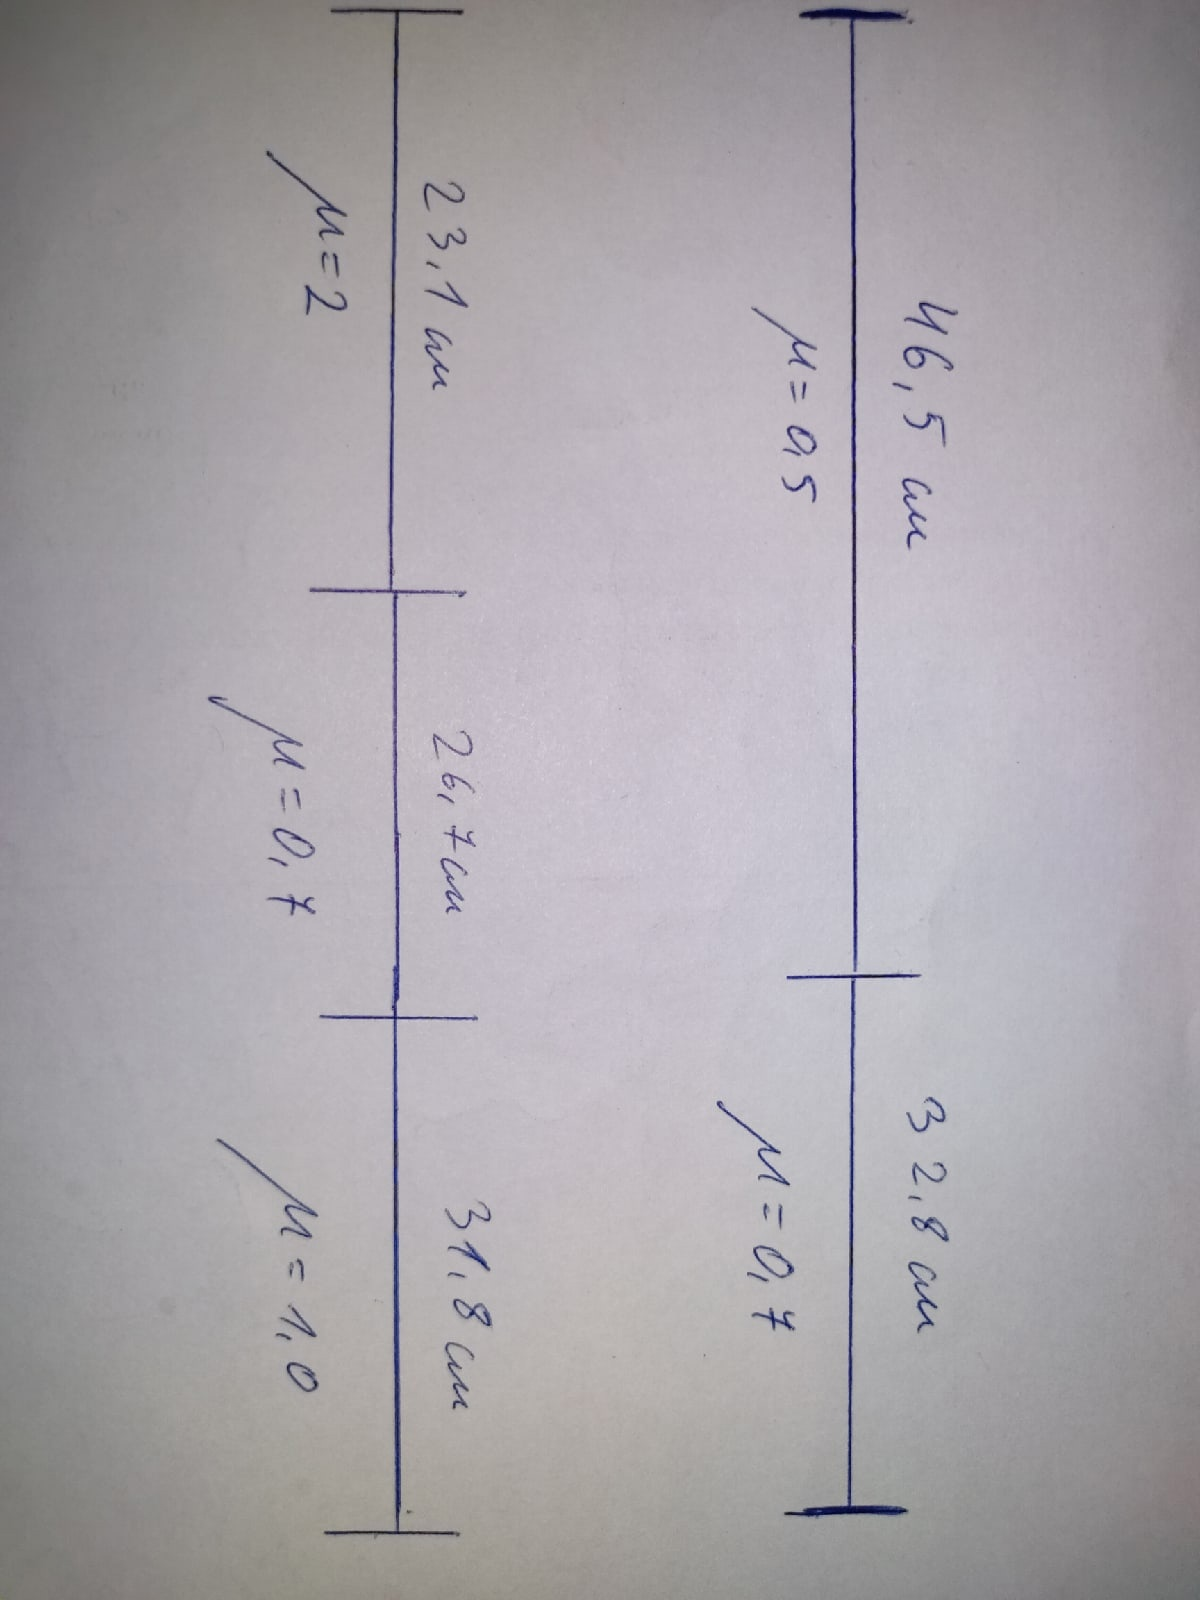
\includegraphics[width = 0.5\textwidth, angle = 90]{UstanovkaScheme.png}
    \caption{Схема установки}
\end{figure}
\begin{figure}[H]\label{fig: UstanovkaPhoto}
    \centering
    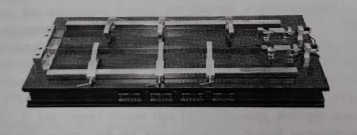
\includegraphics[width = 0.7\textwidth]{UstanovkaPhoto.png}
    \caption{Фото установки}
\end{figure}

Далее, рассчитаем критическую силу для каждого из участков и сравним со значением, полученным на установке
\[P_{кр} = \frac{\pi^2 E J}{(\mu l)^2}\]
\begin{table}[H]\label{tab: P_TeorAndExperiment}
    \centering
    \begin{tabular}{|c|c|c|}
        \hline
        {\color[HTML]{000000} №} & {\color[HTML]{000000} $P_{теор},  Н$} & {\color[HTML]{000000} $P_{эксп},  Н$} \\ \hline
        {\color[HTML]{000000} I.1}  & {\color[HTML]{000000} 18,21}  & {\color[HTML]{000000} 18,0} \\ \hline
        {\color[HTML]{000000} I.2}  & {\color[HTML]{000000} 111,26} & {\color[HTML]{000000} --}    \\ \hline
        {\color[HTML]{000000} I.3}  & {\color[HTML]{000000} 38,43}  & {\color[HTML]{000000} --}    \\ \hline
        {\color[HTML]{000000} II.4} & {\color[HTML]{000000} 91,85}  & {\color[HTML]{000000} 83,0} \\ \hline
        {\color[HTML]{000000} II.5} & {\color[HTML]{000000} 100,20} & {\color[HTML]{000000} --}    \\ \hline
    \end{tabular}
    \caption{Сравнение теоретических и экспериментальных значений $P_{кр}$}
\end{table}
Рассчитаем погрешности $P_{кр}$ учитывая, что 
\[\sigma_l = 5 \cdot 10^{-4} \text{ м}; \text{ } \sigma_b = 5 \cdot 10^{-5} \text{ м};\ text{ } \sigma_h = 10^{-5} \text{ м}\]
\[P = f(h, b, l), \quad \sigma_{P}^2 = \sum (\frac{\partial f}{\partial x_i})^2 \cdot \sigma_{x_i}^2\]
\[\varepsilon_P^2 = \varepsilon_b^2 + 9\varepsilon_h^3 + 4\varepsilon_l^2\]


\begin{table}[H]\label{tab: Pogreshnost}
    \centering
    \begin{tabular}{|c|c|c|}
        \hline
        {\color[HTML]{000000} №} & {\color[HTML]{000000} $P_{теор},  Н$} & {\color[HTML]{000000} $\varepsilon_P, \text{ \%}$} \\ \hline
        {\color[HTML]{000000} I.1}  & {\color[HTML]{000000} $18,21 \pm 0,55$}  & {\color[HTML]{000000} 3,04} \\ \hline
        {\color[HTML]{000000} I.2}  & {\color[HTML]{000000} $111,26 \pm 3,37$} & {\color[HTML]{000000} 3,03} \\ \hline
        {\color[HTML]{000000} I.3}  & {\color[HTML]{000000} $38,43 \pm 1,16$}  & {\color[HTML]{000000} 3,03} \\ \hline
        {\color[HTML]{000000} II.4} & {\color[HTML]{000000} $91,85 \pm 2,76$}  & {\color[HTML]{000000} 3,01} \\ \hline
        {\color[HTML]{000000} II.5} & {\color[HTML]{000000} $100,20 \pm 3,03$} & {\color[HTML]{000000} 3,02} \\ \hline
    \end{tabular}
    \caption{Результаты расчета $P_{кр}$ с учётом погрешностей}
\end{table}

\textbf{Вывод:} В данной работе исследовались основные понятия теории устойчивости стержней, в качестве стержней использовались металлические линейки. Для каждой из линеек, в зависимости от способа закрепления её концов, была рассчитана критическая сила $P_{кр}$, для двух из линеек были получены и значения этих сил экспериментально, таким образом была проверена справедливость формулы Эйлера.

\end{document}
